% RECOMMENDED %%%%%%%%%%%%%%%%%%%%%%%%%%%%%%%%%%%%%%%%%%%%%%%%%%%
\documentclass[graybox,vecarrow]{styles/svmult}
\usepackage{etex}

\usepackage[all]{xy}

% choose options for [] as required from the list
% in the Reference Guide

\usepackage{mathptmx}       % selects Times Roman as basic font
\usepackage{helvet}         % selects Helvetica as sans-serif font
\usepackage{courier}        % selects Courier as typewriter font
%\usepackage{type1cm}        % activate if the above 3 fonts are
                            % not available on your system

\usepackage{makeidx}         % allows index generation
\usepackage{graphicx}        % standard LaTeX graphics tool
                             % when including figure files
\usepackage{multicol}        % used for the two-column index
\usepackage[bottom]{footmisc}% places footnotes at page bottom

% see the list of further useful packages
% in the Reference Guide

\makeindex             % used for the subject index
                       % please use the style svind.ist with
                       % your makeindex program
%\usepackage{showidx}




\usepackage{url}
\usepackage{natbib}
%\usepackage[margin=25mm]{geometry}


\usepackage{amsmath,amssymb,amsfonts}
%\renewcommand{\vec}[1]{\overrightarrow{#1}}
\DeclareMathAlphabet{\mathcal}{OMS}{cmsy}{m}{n} % use '{b}' instead of '{m}' to make bold
\usepackage{wrapfig}
\usepackage{subfig}
\usepackage{drs}
\renewcommand\drsalignment{l}
\newcommand\drsarraystretch{1.05}
\usepackage{parskip}
\usepackage{xspace}
\usepackage{tikz}
\usepackage{tikz-qtree}
\usepackage{styles/modcov}
\usepackage{esvect}

\newcommand\pred[2]{#1\ensuremath{_{#2}}}
\newcommand\POSPRED[1]{\ensuremath{P\hspace{-0.5px}O\hspace{-0.5px}S(#1)}}
\newcommand\NEGPRED[1]{\ensuremath{N\hspace{-0.5px}E\hspace{-0.5px}G(#1)}}

\newcommand{\entpairex}[3]{
  \begin{covex}\label{#1}
    \begin{itemize} \itemsep -4pt
      \item[{\it p:}] #2
      \item[{\it h:}] #3
    \end{itemize}
  \end{covex}
}

\newcommand\unboxedifdrs[2]
  {\mbox{\let\drsboxalignv=c #1 {\large\ {$\Rightarrow\!\,$}\ } #2}}

\pagestyle{empty}

\begin{document}

\title*{A formal approach to linking logical form and vector-space lexical semantics}
% Use \titlerunning{Short Title} for an abbreviated version of
% your contribution title if the original one is too long
\author{Dan Garrette, Katrin Erk, and Raymond Mooney}
% Use \authorrunning{Short Title} for an abbreviated version of
% your contribution title if the original one is too long
\institute{Dan Garrette \at University of Texas at Austin, \email{dhg@cs.utexas.edu}
\and Katrin Erk \at University of Texas at Austin \email{katrin.erk@mail.utexas.edu} 
\and Raymond Mooney \at University of Texas at Austin \email{mooney@cs.utexas.edu}}

\maketitle


%\abstract{
%  First-order logic provides a powerful and flexible mechanism for  representing natural language semantics.  However, it is an open  question of how best to integrate it with uncertain, weighted  knowledge, for example regarding word meaning. 
%This paper describes a mapping between predicates of logical form and points in a vector space. This mapping is then used to project distributional inferences to inference rules in logical form. We then describe first steps of an approach that uses this mapping to recast first-order semantics into the probabilistic models that are part of Statistical Relational AI. Specifically, we show how Discourse Representation Structures can be combined with distributional models for word meaning inside a Markov Logic Network and used to successfully  perform inferences that take advantage of logical concepts such as  negation and factivity as well as weighted information on word   meaning in context.}



\section{Introduction}

Logic-based \index{logical semantics} 
representations of natural language meaning have a long history
\citep{montague:tj1970,kamp:book93}\nocite{thomason:book1974}.
Representing the meaning of language in a first-order logical form is appealing
because it provides a powerful and flexible way to express even complex
propositions. However, systems built solely using first-order logical forms tend
to be very brittle as they have no way of integrating uncertain knowledge.
They, therefore, tend to have high precision at the cost of low recall
\citep{bos:emnlp2005}.

Recent advances in computational linguistics have yielded robust methods that
use statistically-driven weighted models.  For example, distributional
\index{distributional semantics}
models of word meaning have been used successfully to judge paraphrase
appropriateness by representing the meaning of a word in context as a point in a
high-dimensional semantics space
\citep{erk:emnlp2008,thater:acl2010,reisinger:naacl2010,dinu:emnlp2010,vandecruys:emnlp2011}.
However, these models only address word meaning, and do not
address the question of providing meaning representations for complete
sentences. It is a long-standing open question how best to
integrate the weighted or probabilistic information coming from such modules
with logic-based representations in a way that allows for reasoning over both. 
See, for example, \citet{hobbs:alj93}.

The goal of this work is to establish a formal system for combining
logic-based meaning representations with weighted information into a single
unified framework.  This will allow us to obtain the best of both situations: we
will have the full expressivity of first-order logic and be able to reason with
probabilities.  We believe that this will allow for a more complete and robust
approach to natural language understanding.

While this is a large and complex task, this paper proposes first steps toward
our goal by presenting a mechanism for injecting distributional word-similarity
information from a vector space into a first-order logical form.  We
define a mapping from predicate symbols of logical form to points in
vector space. Our main aim in linking logical form to a vector
 space in this paper is to project inferences from the vector space to
logical form. The inference rules that we use are based on
substitutability. In a suitably constructed distributional
representation, distributional similarity between two words or
expressions $A$ and $B$ indicates
that $B$ can be substituted for $A$ in text~\citep{lin:nlej2001}. This can be described through an inference rule $A \to B$. Distributional
information can also be used to determine the degree $\eta$ to which the rule applies in a
given sentence context
\citep{SzpektorEtAl:08,mitchell:acl2008,erk:emnlp2008,thater:acl2010,reisinger:naacl2010,dinu:emnlp2010,vandecruys:emnlp2011}. This
degree $\eta$ can be used as a weight on the inference rule $A\to B$. 

In this paper, we first present our formal framework for projecting inferences
from vector space to logical form.  We then show how that framework can be
applied to a real logical language and vector space to address issues of
ambiguity in word meaning.  Finally, we show how the weighted inference rules
produced by our approach interact appropriately with the first-order logical
form to produce correct inferences.

Our implementation uses Markov Logic Networks (MLN) \citep{richardson:mlj06} as
the underlying engine for probabilistic inference.  We are able to demonstrate
that an MLN is able to properly integrate the first-order logical representation
and weighted inference rules so that inferences involving correct word sense are
assessed as being highly probable, inferences involving incorrect word sense are
determined to be low probability, and inferences that violate hard logical rules
are determined to have the lowest probability.

\section{Background}

\textbf{Textual entailment.}
\index{Recognizing Textual Entailment}
Recognizing Textual Entailment (RTE) is the task of determining whether one
natural language text, the {\it premise}, implies another, the {\it hypothesis}.
For evaluation of our system, we have chosen to use a variation on RTE in which
we assess the relative probability of entailment for a of set of hypotheses.

We have chosen textual entailment as the mode of evaluation
for our approach because it offers a good framework for testing whether a system
performs correct analyses and thus draws the right inferences from a given text.
As an example, consider \eqref{ex:backgound-rte} below.    
\begin{covex}\label{ex:backgound-rte}
\begin{itemize} \itemsep -3pt
  \item[{\it p:}]~~~    The spill left a stain.
  \item[{\it h1:}]~~~~The spill resulted in a stain.
  \item[{\it h2*:}]~~~~The spill fled a stain.
  \item[{\it h3*:}]~~~~The spill did not result in a stain.
\end{itemize}
\end{covex}
Here, hypothesis {\it h1} is a valid entailment, and should be judged to have
high probability by the system.  Hypothesis {\it h2} should have lower probability since
it uses the wrong sense of {\it leave} and {\it h3} should be low probability
because the logical operator $not$ has reversed the meaning of the premise
statement.

% For example, to test whether a system correctly handles implicative verbs, one
% can use the \emph{premise} $p$ along with the \emph{hypothesis} $h$ in
% \eqref{ex:imp-fact-nested} below. If the system analyses the two sentences
% correctly, it should infer that $h$ holds.
While the most prominent forum using textual entailment is the Recognizing
Textual Entailment (RTE) challenge \citep{dagan:rte2005}, the RTE datasets do
not test the phenomena in which we are interested. For example, in order to
evaluate our system's ability to determine word meaning in context, the RTE pair
would have to specifically test word sense confusion by having a word's context
in the hypothesis be different from the context of the premise.  However, this
simply does not occur in the RTE corpora.  In order to properly test our
phenomena, we construct hand-tailored premises and hypotheses based on
real-world texts.

\vspace{2mm}
\textbf{Logic-based semantics.}
\index{logical semantics}
\index{Discourse Representation Theory}
Boxer \citep{bos:coling2004} is a software package for wide-coverage semantic
analysis that provides semantic representations in the form of Discourse
Representation Structures \citep{kamp:book93}. It builds on the C\&C CCG parser
\citep{clark:acl04}.

\citet{bos:emnlp2005} describe a system for Recognizing Textual Entailment
(RTE) that uses Boxer to convert both the premise and hypothesis of an RTE pair
into first-order logical semantic representations and then uses a theorem prover
to check for logical entailment. 
% \citet{bos:trec2006} varies this model in order
% to use Boxer in a question answering setting by using Boxer to generate a
% logical representation of a document and a question and attempting to unify the
% two to find an answer to the question.


\vspace{2mm}
\noindent\textbf{Distributional models for lexical meaning.} 
\index{distributional semantics} Distributional
models describe the meaning of a word through the context in which it
appears~\citep{landauer97:solution,lund96:producing}, where contexts can be
documents, other words, or snippets of syntactic structure. Based on
the hypothesis that words that are similar in meaning will occur in
similar contexts~\citep{harris:wj1954,firth:slaj1957}, distributional
models predict semantic similarity between words based on
distributional similarity. They can be learned in an unsupervised fashion.
Recently distributional models have been used to predict the applicability of
paraphrases in context \citep{erk:emnlp2008,thater:acl2010,reisinger:naacl2010,dinu:emnlp2010,vandecruys:emnlp2011}.
For example, in ``The spill left a stain'', {\it result in} is a better
paraphrase for {\it leave} than {\it flee}, because of the context of {\it spill}
and {\it stain}.  In the sentence ``The suspect left the country'', the
opposite is true: {\it flee} is a better paraphrase. Usually, the distributional
representation for a word mixes all its usages (senses). For the paraphrase
appropriateness task, these representations are then reweighted, extended, or
filtered to focus on contextually appropriate usages.


\vspace{2mm}
\noindent\textbf{Markov Logic.} 
\index{Markov logic}

In order to perform logical inference with weights, we draw
from the large and active body of work related to Statistical Relational AI
\citep{getoor:book2007}.  Specifically, we make use of Markov Logic Networks
(MLNs) \citep{richardson:mlj06} which employ weighted graphical models to
represent first-order logical formulas. MLNs are appropriate for our approach
because they provide an elegant method of assigning weights to first-order
logical rules, combining a diverse set of inference rules, and performing
probabilistic inference. \index{probabilistic inference}

An MLN consists of a set of weighted first-order clauses.  It provides a way of
softening first-order logic by making situations in which not all clauses are
satisfied less likely, but not impossible \citep{richardson:mlj06}. More
formally, if $X$ is the set of all propositions describing a world (i.e. the
set of all ground atoms), $\mathcal{F}$ is the set of all clauses in the MLN,
$w_i$ is the weight associated with clause $f_i \in \mathcal{F}$,
$\mathcal{G}_{f_i}$ is the set of all possible groundings of clause $f_i$, and
$\mathcal{Z}$ is the normalization constant, then the probability of a
particular truth assignment $\mathbf{x}$ to the variables in $X$ is defined as:
\[ P(X = \mathbf{x}) = \frac{1}{\mathcal{Z}} \exp\left(\sum_{f_i \in
\mathcal{F}} w_i \sum_{g \in \mathcal{G}_{f_i}}g(\mathbf{x}) \right) =
\frac{1}{\mathcal{Z}} \exp\left(\sum_{f_i \in \mathcal{F}} w_i n_i(\mathbf{x})
\right) \] where $g(\mathbf{x})$ is 1 if $g$ is satisfied and
0 otherwise, and $n_i(\mathbf{x})= \sum_{g\in \mathcal{G}_{f_i}}g(\mathbf{x})$
is the number of groundings of $f_i$ that are satisfied given the current truth
assignment to the variables in $X$. This means that the probability of a truth
assignment rises exponentially with the number of groundings that are satisfied.

Markov Logic has been used previously in other NLP applications
(e.g. \citet{poon:emnlp2009}).  However, this paper differs in that it is an
attempt to represent deep logical semantics in an MLN.

While it is possible to learn rule weights in an MLN directly from training data,
our approach at this time focuses on incorporating weights computed
by external knowledge sources.  Weights for word meaning rules are computed from
the distributional model of lexical meaning and then injected into the MLN. 
Rules governing implicativity are given infinite weight (hard constraints).

We use the open source software package Alchemy \citep{kok:tr05} to perform MLN
inference.

% logical language
\newcommand{\loglang}{\ensuremath{{\cal{L}}}\xspace}
% predicate symbols
\newcommand{\predsym}[1]{\ensuremath{{\cal{P}}_{#1}}\xspace}
% similarity function
\newcommand{\simfunc}{\ensuremath{\mathrm{sim}}\xspace}

\section{Linking logical form and vector spaces}
\label{sec:interface}
\index{vector space}

In this section we define a link between logical form and vector space
representations through a mapping function that connects predicates in logical
form to points in vector space. \citet{gardenfors:book2004} uses the
interpretation function for this purpose, such that logical formulas are
interpreted over vector space representations. However, the 
\emph{conceptual spaces} that he uses are not distributional. Their
dimensions are qualities, like the hue and saturation of a color or
the taste of 
a fruit. Points in a conceptual space are, therefore, potential entities. In
contrast, the vector spaces that we use are distributional in nature, and, therefore, cannot be interpreted as potential
entities. A point in such a space is a potential word, defined through
its observed contexts. For
this reason, we define the link between logical form and vector space through a
second mapping function independent of the interpretation function, which we
call the \emph{lexical mapping} function.

\subsection*{Lexical mapping and inference projection} 

% [TODO: \\vec is making vectors bold instead of using an overarrow]
% KE: leave them bold. this is due to mathptmx.
% Probably too much of a nuisance to change back, plus it 
% might be inconsistent with other papers in the book to have an overarrow.

Let $V$ be a vector space whose dimensions stand for elements of  textual
context. We also write $V$ for the set of points in the space. We assume that
each word is represented as a point in vector space.\footnote{The assumption of
a single vector per word is made for the sake of simplicity. If we want to cover
models in which each word is represented through multiple
vectors~\citep{reisinger:naacl2010,dinu:emnlp2010}, this can be done through
straightforward extensions of the definitions given here.}
The central relation in vector spaces is semantic similarity. We represent this
through a \textit{similarity function} \[\simfunc: V \times V \to [0,1] \] that
maps each pair of points in vector space to their degree of similarity. While
most similarity functions in the literature are symmetric, such that 
$\simfunc(\vec v, \vec w) = \simfunc(\vec w, \vec v)$, our definition also
accommodates asymmetric similarity measures like \citet{kotlerman:nlej2010}.

We link logical form and a vector space through a function that maps every
predicate symbol to a point in space. Let \loglang be a logical language. For
each $n \ge 0$, let the set of $n$-ary predicate symbols of \loglang be
$\predsym{\loglang}^n$, and let $\predsym{\loglang} = \cup_{n \ge 0}
\predsym{\loglang}^n$. Let $V$ be a vector space. Then a \emph{lexical mapping
function} from \loglang to $V$ is a function $\ell:
\predsym{\loglang} \to V$.



A central property of distributional vector spaces is that they can predict
similarity in meaning based on similarity in observed
contexts~\citep{harris:wj1954}. \citet{lin:nlej2001} point out that in
suitably constrained distributional representations, distributional
similarity indicates substitutability in text. If two words $v$ and
$w$ are similar in their observed contexts, then $w$ can be
substituted for $v$ in texts. This can be written as an
inference rule $v \to w$, weighted by $\simfunc(\vec v, \vec w)$.

We use this same idea to project inference rules from vector space to logical
form through the lexical mapping function. If the lexical mapping function maps
the $n$-ary predicate $P$ to $\vec v$ and the $n$-ary predicate $Q$ to $ \vec w$,
and $\simfunc(\vec v, \vec w) = \eta$, then we obtain the weighted inference
rule $\forall x_1, \ldots, x_n[ P(x_1, \ldots, x_n) \to Q(x_1, \ldots x_n) ]$
with weight $\eta$. More generally, let \loglang be a logical language with
lexical mapping $\ell$ to a vector space $V$. Let \simfunc{} be the similarity
function on $V$. For all $Q \in \predsym\loglang$ and ${\cal Q} \subseteq
\predsym\loglang$, let $\zeta(Q, {\cal Q}) \subseteq {\cal Q}$. Then the
\emph{inference projection} for the predicate $P \in \predsym{\loglang}^n$ is
\begin{align*}
&\Pi_{\simfunc, \zeta, \ell}(P) = \{ (F, \eta) \mid \exists Q \in \zeta(P, \predsym{\loglang}^n)\:[ \\ 
& \hspace{125px} F = \forall x_1, \ldots, x_n[P(x_1, \ldots, x_n) \to Q(x_1, \ldots, x_n)], \\
& \hspace{125px} \eta = \simfunc\big(\ell(P), \ell(Q)\big) ~] \}
\end{align*}
That is, the inference projection for $P$ is the set of all weighted inference
rules $(F, \eta)$ predicted by the vector space that let us infer some
other predicate $Q$ from $P$. Additionally, we may have information on the 
inferences that we are willing to project that is not encoded in the vector 
space. For example we may only want to consider
predicates $Q$ that stand for paraphrases of $P$. For this reason, the
function $\zeta$ can be used to limit the predicates $Q$ considered for the right-hand
sides of rules. If $\zeta(P, \predsym\loglang^n) =
\predsym\loglang^n$, then a rule will
be generated for every $Q \in \predsym{\loglang}^n$. 


\subsection*{Addressing polysemy}
\index{polysemy}

When a word is polysemous, this affects the applicability of vector
space-based inference rules. Consider the rule $\forall e[fix(e) \to
correct(e)]$ (any fixing event is a correcting event): This rule
applies in contexts like ``fix a problem'', but not in contexts like
``fix the date''. We therefore need to take context into account when
considering inference rule applicability. We do this by computing
vector representations for word meaning in context, and predicting
rule applicability based on these context-specific vectors. We follow
the literature on vector space representations for word meaning in context
\citep{erk:emnlp2008,thater:acl2010,reisinger:naacl2010,dinu:emnlp2010,vandecruys:emnlp2011}
in assuming that a word's context-specific meaning is a function of its
out-of-context representation and the context. The context may consist
of a single item or multiple items, and (syntactic or semantic) relations to the
target word may also play a
role~\citep{erk:emnlp2008,thater:acl2010,vandecruys:emnlp2011}. 

We first define what we mean by a context. Given a vector space $V$ and a finite
set $R$ of semantic relations, the set \textit{$C(V, R)$ of contexts over $V$
and $R$} consists of all finite sets of pairs from $V \times R$.  That is, we
describe the context in which a target word occurs as a finite set of pairs
$(\vec v, r)$ of a context item $\vec v$ represented as a point in vector space,
and the relation $r$ between the context item and the target.
For a word $w$ in a context $c \in C(V, R)$, the context-specific meaning $\vec
w_c$ of $w$ is a function of the out-of-context vector $\vec w$ for $w$ and the
context $c$:
\[\vec w_c = \alpha(\vec w, c)\] The function $\alpha$ is a
\emph{contextualization function} with signature $\alpha: V \times C(V, R) \to
V$.

This definition of contextualization functions is similar to the framework of
\citet{mitchell:acl2008}, who define the meaning $\vec p$ of a two-word phrase
$p = vw$ as a function of the vectors for $v$ and $w$, and their syntactic
relation $r$ in the text: $\vec p = f(\vec v, \vec w, r, K)$,  where $f$ is some
function, and $K$ is background knowledge. However, we use contextualization
functions to compute the meaning of a word in context, rather than the meaning
of a phrase. We map predicate symbols to points in space, and predicate symbols
need to map to word meanings, not phrase meanings. Also, Mitchell and Lapata
only consider the case of two-word phrases, while we allow for arbitrary-size
contexts.


In existing approaches to computing word meaning in context, bag-of-words
representations or syntactic parses of the sentence context are used to compute
the contextualization. In contrast, we use the logical form representation,
through a function that maps a logic formula to a context in $C(V, R)$.  Given a
logical language \loglang, a vector space $V$, and set $R$ of semantic
relations, a \textit{context mapping} is a function that computes the context $c
\in C(V, R)$ of a predicate $P$ in a formula $G$ as \[c = \kappa(P, G)\] The
signature of a context mapping function is $\kappa:
\predsym{\loglang} \times \loglang \to C(V, R)$.

We can now compute a context-specific vector space representation $\vec{w}_{P,
G}$ for a predicate $P$ in a formula $G$ from the context-independent vector
$\ell(P)$ and the context $\kappa(P, G)$. It is \[\vec{w}_{P, G} =
\alpha\big(\ell(P), \kappa(P, G)\big)\]

To obtain an inference projection for $P$ that takes into account its context in
the formula $G$, we adapt the lexical mapping function. Given a lexical mapping
$\ell$, let $\ell_{[Q/\vec{v}]}$ be the function that is exactly like $\ell$
except that it maps $Q$ to $\vec v$. Let $\Pi_{\simfunc, \zeta, \ell}$ be an
inference projection for vector space $V$ and logical language $\loglang$, let
$\alpha$ be a contextualization function on $V$ and $R$, and $\kappa$ a context
mapping from \loglang to $C(V, R)$. Then the \textit{contextualized inference
projection} for predicate $P \in \predsym{\loglang}^n$ in formula $G \in
\loglang$ is \[ \Pi^G_{\simfunc, \zeta, \ell}(P) = \Pi_{\simfunc, \zeta,
  \ell_{[P/\alpha(\ell(P), \kappa(P, G))}}(P)
\] In this contextualized inference projection, any rule $\forall x_1,\ldots,x_n [P(
x_1,\ldots,x_n) \to Q(x_1,\ldots,x_n)]$ is weighted by similarity $\simfunc(\alpha(\ell(P), \kappa(P,
G)), \ell(Q))$ between the context-specific vector for $P$ and the vector for
$Q$. This follows common practice in vector space models of word meaning in
context of computing a context-specific representation of the target, but not
the paraphrase candidate. But if the paraphrase candidate is polysemous, it may
be useful to compute a representation for it that is also specific to the
sentence context at hand~\citep{erk:acl2010}.  We can do this by defining a
lexical mapping $\gamma^{P, G}$ specific to predicate $P$ and formula $G$ by
$\gamma^{P, G}(Q) = \alpha\big(\ell(Q), \kappa(P, G)\big)$. Then we can compute
the contextualized inference projection of $P$ as $\Pi^G_{\simfunc, \zeta,
\ell}(P) = \Pi_{\simfunc, \zeta, \gamma^{P, G}}(P)$.

In computational semantics, polysemy is mostly addressed by using multiple
predicates. For example, for the noun ``bank'' there would be predicates
bank$_1$, bank$_2$ to cover the financial and riverside senses of the word. In
contrast, we use a separate predicate for each word token, but these 
predicates are not associated with any particular fixed senses. Instead, we vary
the lexical mapping of a predicate based on the formula that it appears in: 
A predicate $P$ in
a formula $G$ is mapped to the vector $\alpha\big(\ell(P), \kappa(P, G)\big)$,
which depends on $G$. We make this change for two reasons. First, a system that
uses distinct predicates bank$_1$, bank$_2$ has to rely on an external word
sense disambiguation system that decides, during semantics construction, which
of the senses to use. In contrast, we determine lexical meaning based on the
overall semantic representation of a sentence, directly linking sentence
semantics and lexical semantics. Second, in the case of polysemy, the senses to
distinguish are not always that clear. For example, for a noun like ``onion'',
should the vegetable sense and the plant/bulb sense be
separate~\citep{krishnamurthy:chj2000}? Through the vector space model, we
can model word meaning in context without ever referring to distinct dictionary
senses~\citep{erk:gems2010}. 
But if we do not want to consider a fixed list of senses for a word
$w$, then we also cannot represent its meanings through a fixed list of predicates.

\section{Transforming natural language text to logical form}
\index{Boxer}
\index{Discourse Representation Theory}

In transforming natural language text to logical form, we build on the software
package Boxer \citep{bos:coling2004}. Boxer
is an extension to the C\&C parser \citep{clark:acl04} that transforms a parsed
discourse of one or more sentences into a semantic representation.  Boxer
outputs the meaning of each discourse as a Discourse Representation Structure
(DRS) that closely resembles the structures described by \citet{kamp:book93}.

We chose to use Boxer for two main reasons.  First, Boxer is a wide-coverage
system that can deal with arbitrary text.
% that is able to return a reasonable logical representation of most English
% sentences.  Since our goal is to work with actual texts, it is critical that
% we have a wide-coverage semantic parser.  If we did not, then we would be
% unable to deal with any but the simplest texts.
Second, the DRSs that Boxer produces are close to the standard first-order
logical forms that are required for use by the MLN software package Alchemy.
Our system interprets discourses with Boxer, augments the resulting logical
forms by adding inference rules, and outputs a format that the MLN
software Alchemy can read.

\section{Ambiguity in word meaning}
\index{lexical ambiguity}

In order for our system to be able to make correct natural language inferences,
it must be able to handle paraphrasing.  For example, in order to license the
entailment pair in (\ref{ex:syn-hyp-pos}), the system must recognize that
``owns'' is a valid paraphrase for ``has'', and that a ``car'' is type of
``vehicle'':

\entpairex{ex:syn-hyp-pos}{Ed owns a car.}{Ed has a vehicle.}

We address this problem as described in Section~\ref{sec:interface}: 
We use distributional information to
generate inferences stating, for example,  that ``has'' can be substituted for
``owns''. This inference is weighted by the degree to which 
``owns'', in the context in which it is used in
(\ref{ex:syn-hyp-pos}), is similar to ``has''. To integrate these
inference rules with the logical form representations of sentences
like (\ref{ex:syn-hyp-pos}), we use the formalism introduced in
Section \ref{sec:interface}. We now describe how we instantiate it in
the current paper.

% KE: weird paragraph, sounds like we had not introduced the notion
% of inference rules based on distributional information
% before. Instead, point to section 3. 
% Perhaps the most natural fit for our system of projecting distributional
% information into logical forms is trying to generate inference rules to address
% lexical ambiguity.  For any natural language sentence $A$, a word $v$ in $A$ may
% be replaced by a synonym of $v$, $w$, resulting in a new sentence $A'$.  The
% degree to which $A'$ means the same thing as $A$ is determined by how well $w$
% fits the context of $v$ in $A$.  Thus, in order to capture the
% strength of our conviction that
% $A$ entails $A'$, we want to generate an inference rule stating that $v$ implies
% $w$ to the degree that that $w$ fits the context of $v$.


First, we generate a vector space $V$.  We have chosen to implement a very
simple vector space based on a bag-of-words representation of context.  To ensure that the entries in the vector
space correspond to the predicates in our logical forms, we first lemmatize all
sentences in our corpus using the same lemmatization process as Boxer.
The features used by $V$ are the $N$ most frequent lemmas, excluding stopwords.  
To calculate the vector in $V$ for a lemma, we count the number of times the lemma appears in the same sentence
as each feature, and then calculate the point-wise mutual information (PMI)
between the lemma and each feature.  The resulting PMI values for each feature
are used as the vector for the lemma.

As the \emph{similarity function} \simfunc on our vector space, we use cosine
similarity. For two vectors $\vec v$ and $\vec w$, their similarity is 
\[ \simfunc(\vec v, \vec w) = cosine(\vec v, \vec w) = \frac{\vec v \cdot \vec
w}{\|\vec v\|~\|\vec w\|}\]

Logical forms in our system are generated by Boxer, so our logical language
\loglang is the set of formulas that may be returned from Boxer (modulo
some modifications described in Section~\ref{sec:implicativity}).  Likewise, the
set of predicate symbols $\predsym{\loglang}$ are the predicates generated by
Boxer. Boxer's predicates, as represented by the {\tt pred} relation in Boxer's
Prolog output,\footnote{See
\url{http://svn.ask.it.usyd.edu.au/trac/candc/wiki/DRSs} for the detailed
grammar of Boxer DRS output.} consist of a word lemma and a token index
indicating the original token that generated that predicate.  
% lexical mapping maps to vectors, not words!
Our \emph{lexical mapping} function maps each predicate symbol to the
vector that represents the lemma portion of the predicate.

In order to assess the similarity between a word's context and a possible
replacement word, we must define a \textit{context mapping} that generates a
context from a predicate $P \in \predsym{\loglang}$ and a formula $G \in
\loglang$.  For the current paper we use the simplest possible
definition for $\kappa$, which ignores semantic relations. We define 
% We can define our context mapping as a function that maps $P$ to the set of
% vectors representing the other predicates in $G$ along with the relations that
% connect them.
% \begin{align*}
% \kappa(P,G) = \{ (r_i, \ell(Q)) ~| 
% &~Q \text{ is a predicate found in } G, \\
% &~r_i = \text{the relation connecting } P \text{ and } Q, \text{ and } \\
% &~Q \neq P \}
% \end{align*}
% However, in our current scenario, the only ``relation'' we use is the relation
% of being in the same sentence.  So, we are defining 
the context of $P$ as the
vectors of all predicates $Q$ that occur in the same sentence as $P$.
Since every predicate in a logical form returned by Boxer is indexed
with the sentence from which it was generated, we can define a simple context
mapping that defines a predicate's context solely in terms of the other
predicates generated by Boxer for that sentence.
\begin{align*}
\kappa(P,G) = \{ (same\text{-}sentence, \ell(Q)) ~|
&~Q \text{ is a predicate found in } G, \\
&~Q\text{'s sentence index} = P\text{'s sentence index}, \text{ and } \\
&~Q \neq P \}
\end{align*}
Note that the only predicates $Q$ that are used are those derived from the
lemmas of words found in the text.  Meta-predicates representing relations such
as $agent$, $patient$, and $theme$ are not included.

The context mapping $\kappa$ computes a context for a predicate $P$
occurring in a formula $G$. Next we require a 
\textit{contextualization function} that uses the context returned by
$\kappa$ to compute a context-specific vector for $P$. Again we use
the simplest instantiation possible. Our contextualization
function just computes the sum of the vectors for each lemma in the context \[ \alpha(\vec v,
c) = \sum_{(r_i, \vec w_i) \in c} \vec w_i \]  Other, more complex
instantiations of $\kappa$ and $\alpha$ are possible. We comment on
this further in Section~\ref{sec:future}. 

Based on these definitions, we compute the \textit{contextualized
inference projection} $\Pi^G_{\simfunc,\zeta,\ell}(P)$, the set of weighted
inference rules mapping predicate $P$ to its potential replacements,
as described in Section~\ref{sec:interface}.

Finally, in order to limit the number of inference rules generated in the
inference projection, we define a restriction function $\zeta$ that specifies,
for a predicate $P \in \predsym{\loglang}^n$, which of the predicates in
$\predsym{\loglang}^n$ may serve as replacements.  Our system uses WordNet
\citep{miller:wordnet2009} to restrict substitutions only to those predicates
representing synonyms or hypernyms of the lemma underlying $P$.  So, for a
predicate $P \in \predsym{\loglang}^n$ and a set of predicates ${\cal Q}
\subseteq \predsym{\loglang}^n$, we define $\zeta$ as \[ \zeta(P,{\cal Q}) = \{
Q \in {\cal Q} ~|~ Q\text{'s lemma is a synonym of, a hypernym of, or equal to
}P\text{'s} \} \]


\subsection*{A lexical ambiguity example}

Assume we have sentence \eqref{ex:lexical-ambiguity}, which is parsed by C\&C
and translated into DRT by Boxer, as shown in Figure
\ref{drs:lexical-ambiguity}.

\vspace{5mm}
\begin{covex}\label{ex:lexical-ambiguity}
\begin{itemize} \itemsep -3pt
  \item[{\it p:}]~~~  A stadium craze is sweeping the country.
  \item[{\it h1:}]~~~~A craze is covering the nation.
  \item[{\it h2*:}]~~~~A craze is brushing the nation.
\end{itemize}
\end{covex}

\begin{figure}
  \centering
  ~~~~~~~~
  \subfloat[Dependency output from C\&C]{\label{drs:lexical-ambiguity-deps}
    \begin{minipage}[c][0.7\width]{0.5\textwidth}
	  %\centering
	    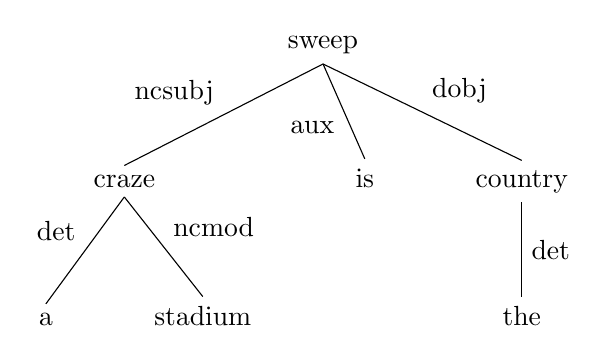
\begin{tikzpicture}[level distance=50pt, sibling distance=30pt]
	      \Tree 
	        [.sweep
	          \edge node[auto=right]{ncsubj}; [.craze  
	            \edge node[auto=right]{det};   [.a ]
	            \edge node[auto=left]{ncmod}; [.stadium ]
	          ]
	          \edge node[auto=right]{aux}; [.is ]
	          \edge node[auto=left]{dobj}; [.country 
	            \edge node[auto=left]{det}; [.the ]
	          ]
	        ]
	    \end{tikzpicture}
		% (ncmod _ craze_2 stadium_1)
		% (det craze_2 A_0)
		% (det country_6 the_5)
		% (dobj sweeping_4 country_6)
		% (aux sweeping_4 is_3)
		% (ncsubj sweeping_4 craze_2 _)
	\end{minipage}
  }
  \subfloat[DRT output from Boxer]{\label{drs:lexical-ambiguity-drs}
    \begin{minipage}[c][0.7\width]{0.5\textwidth}
	  %\centering
		\drs{~x0 x1 e2 x3~}{
		  ~\pred{stadium}{1002}(x0)~ \\
		  ~nn(x0, x1)~ \\
		  ~\pred{craze}{1003}(x1)~ \\
		  ~agent(e2, x1)~ \\
		  ~\pred{sweep}{1005}(e2)~ \\
		  ~event(e2)~ \\
		  ~\pred{country}{1007}(x3)~ \\
		  ~patient(e2, x3)~
		}
	\end{minipage}
  }
  \caption{Dependency parse tree and DRT interpretation of
  the premise in \eqref{ex:lexical-ambiguity}}
  \label{drs:lexical-ambiguity}
\end{figure}

The DRS in Figure \ref{drs:lexical-ambiguity-drs}, a formula of logical language
\loglang, shall be denoted by $G$.  Formula $G$ contains a unary predicate
$sweep_{1005}$.  In order to generate weighted substitution rules for
$sweep_{1005}$, we calculate the {\it contextualized inference projection} of
$sweep_{1005}$: the set of inference rules mapping $sweep_{1005}$ to each
(unary) predicate $Q \in \predsym{\loglang}^1$, with each rule weighted by the
similarity of the vector representing the context of $sweep_{1005}$ in $G$ to
the vector representing the replacement $Q$. This is 
\begin{align*}
&\Pi^G_{\simfunc, \zeta, \ell}(sweep_{1005}) = \\
& \hspace{50px} \{ (F, \eta) \mid \exists Q \in \zeta(P, \predsym{\loglang}^1)~[ \\
& \hspace{110px} F = \forall x.[sweep_{1005}(x) \to Q(x)] \text{ and } \\
& \hspace{110px} \eta = \simfunc\big(\alpha(\ell(sweep_{1005}), \kappa(sweep_{1005}, G)), \ell(Q)\big)~] \}
\end{align*}

Let us assume that our logical language \loglang also includes unary predicates
$cover_{2004}$ and $brush_{3004}$ and that the lemmas {\it cover} and {\it
brush} are known to be synonyms of {\it sweep} (though from different senses). 
In other words, \[ \{ cover_{2004},~ brush_{3004} \} \in \zeta(sweep_{1005},~
\predsym{\loglang}^1) \] So, in the calculation of $\Pi^G_{\simfunc,\zeta
\ell}(sweep_{1005})$, we will generate weighted inference rules $(F,\eta)$ for
both $cover_{2004}$ and $brush_{3004}$.  This will allow us to calculate the
probability of inference for both hypotheses in \eqref{ex:lexical-ambiguity}.

\vspace{8mm}
We look first at $cover_{2004}$.  The rule formula $F$ is instantiated simply as
\[ \forall x.[sweep_{1005}(x) \to cover_{2004}(x)] \]  The weight $\eta$ is the
similarity between the context of $sweep_{1005}$ in $G$, and $cover_{2004}$.
The context vector for $sweep_{1005}$ is calculated as \[
\alpha(\ell(sweep_{1005}), \kappa(sweep_{1005}, G)) \]  Since we defined the
lexical mapping $\ell(P)$ to simply return the vector from $V$ for the lemma
portion of the predicate $P$, $\ell(sweep_{1005}) = \vv{sweep}$ and
$\ell(cover_{2004}) = \vv{cover}$.  

The context of $P$ in $G$, $\kappa(P,G)$ is the set of a set of
predicates and their relations to $P$, so
\begin{align*}
\kappa(sweep_{1005}, G) 
= \{ & (\ell(\pred{stadium}{1002}),~same\text{-}sentence) \} \\
     & (\ell(\pred{craze}{1003}),~same\text{-}sentence), \\ 
     & (\ell(\pred{country}{1007}),~same\text{-}sentence), \\ 
= \{ & (\vv{stadium},~same\text{-}sentence), \\
     & (\vv{craze},~same\text{-}sentence), \\
     & (\vv{country},~same\text{-}sentence) \}
\end{align*}
We defined our contextualization function $\alpha(\vec v, c)$ to be the vector
sum of word vectors from the context $c$, so
\begin{align*}
\alpha(\ell(sweep_{1005}), \kappa(sweep_{1005}, G))
& = \alpha(\vv{sweep},~ \{ 
                (\vv{stadium},~same\text{-}sentence), \\
& \hspace{60px} (\vv{craze},~same\text{-}sentence), \\
& \hspace{60px} (\vv{country},~same\text{-}sentence) \}) \\
& = \vv{stadium} + \vv{craze} + \vv{country}
\end{align*}

Finally, since we have the vector representing the context of $sweep_{1005}$ in
$G$ and the vector representing the replacement predicate $cover_{2004}$, we can
compute the weight, $\eta$ for our inference rule $\forall x.[sweep_{1005}(x)
\to cover_{2004}(x)]$ as
\begin{align*}
& \simfunc\big(\alpha(\ell(sweep_{1005}), \kappa(sweep_{1005}, G)), \ell(Q)\big) \\
& \hspace{120px} = \simfunc\big(\vv{stadium} + \vv{craze} + \vv{country},~ \vv{cover}\big) \\
& \hspace{120px} = cosine\big(\vv{stadium} + \vv{craze} + \vv{country},~ \vv{cover}\big)
\end{align*}
Likewise, the rule for replacing $sweep_{1005}$ by $brush_{3004}$ would be 
$\forall x.[sweep_{1005}(x)$ $\to$ $brush_{3004}(x)]$ weighted by 
$cosine\big(\vv{stadium} + \vv{craze} + \vv{country},~ \vv{brush}\big)$.

Since, $cosine\big(\vv{stadium}$ $+$ $\vv{craze}$ $+$ $\vv{country},~
\vv{cover}\big)$ $>$ $cosine\big(\vv{stadium}$ $+$ $\vv{craze}$ $+$ $\vv{country},~
\vv{brush}\big)$, {\it cover} is considered to be a better replacement for {\it
sweep} than {\it brush} in the sentence ``A stadium craze is sweeping the
country''.  Thus, the rule $\forall x.[sweep_{1005}(x) \to cover_{2004}(x)]$
will be given more consideration during inference, and hypothesis {\it h1} will
be determined to be more probable than {\it h2}.




\subsection*{Hypernymy}

According to our definition of $\zeta$ above, we construct inference rules of
the form $\forall x_1, \ldots, x_n[ P(x_1, \ldots, x_n) \to Q(x_1, \ldots x_n)
]$ where $Q$ is a synonym or hypernym of $P$.  Thus, for two synonyms $A$ and
$B$, we will generate rules $A \to B$ and $B \to A$.  However, for hypernym
relationships, we only construct the inference rule entailing {\it up} the
hierarchy: from the hyponym to the hypernym.  This is important for licensing
correct inferences.  Consider example \eqref{ex:hyp-1}.
\entpairex{ex:hyp-1}{Ed owns a car.}{Ed has a vehicle.}
Here the inference is valid since a {\it car} is a type of {\it vehicle}. 
For this pair, our system will generate the rule $\forall x[car(x) \to
vehicle(x)]$ and assign a weight based on the similarity of the lemma $vehicle$
to the context of $car$ in the premise sentence.  However, an inference in the
reverse direction of \eqref{ex:hyp-1} would be invalid, which is why we do not
generate the reverse inference rule.


%\subsection*{Integration between logical and distributional phenomena}

With hypernymy, we can see how our system naturally integrates logical phenomena
with distributional information.  In example \eqref{ex:hyp-1}, the
distributional similarity between {\it vehicle} and the context of {\it car}
affects the overall probability of inference for the pair.  However, it does not
override the logical requirements imposed by the hypernym relationship: if the
premise and hypothesis were reversed then it would not matter how similar the
words were since the inference would be impossible.

The logical rules generated for hypernyms work properly with other logical
aspects as well.  For example, in \eqref{ex:hyp-3} below we can see that the
direction of entailment along the hypernym hierarchy is reversed when the words
appear in negative contexts.  Our system handles this correctly.

% Above, we stated that the entailment in \eqref{ex:hyp-1} was licensed because a
% {\it car} is a type of {\it vehicle} and we can entail from a subset to a
% superset.  In fact, the situation is complicated a bit because the direction of
% entailment is actually dictated by the polarity of the context in which the
% words appear.
% 
% Consider example \eqref{ex:hyp-3} below
\entpairex{ex:hyp-3}{Ed does not own a vehicle.}{Ed does not have a car.}
% This entailment is valid despite the fact that we are entailing from {\it
% vehicle} to {\it car}, the opposite direction as in example \eqref{ex:hyp-1}.
% The difference is that in \eqref{ex:hyp-1}, the words appeared in a {\it
% positive context} while in \eqref{ex:hyp-3} they appear in a {\it
% negative context} since they are embedded under a single negation.
% 
% However, the approach that we have chosen to take handles this interaction
% naturally.  The softened inference rules we generate for hypernym relationships
% may lower the probability of entailment versus a similar hard rule (when the
% weight is less than 1), but if an entailment rule does not fit the polarity of
% the context, then it will not raise the probability of entailment.
% 
% In addition to negation, other linguistic constructs such as quantifiers and
% implicative verbs may affect the polarity of a context
% \citep{maccartney:iwcs2009}.  Our system handles all equally well.

\section{Implicativity}
\label{sec:implicativity}
\index{implicativity}
\index{factivity}

Implicativity and factivity are concerned with analyzing the truth conditions of
nested propositions \citep{nairn:icos2006}.  
For example, in the premise of the entailment pair shown in example 
\eqref{ex:imp-fact-nested} below, the {\it locking} is the event that Ed
{\it forgot to} do, meaning that it did not happen.  In example
\eqref{ex:hope-build}, {\it build} is the main verb of the complement of 
{\it hope}, so we cannot infer that the {\it building} event occurred, nor 
can we infer that it did not occur.  Correctly recognizing nested
propositions and analyzing their contexts is necessary for preventing
the licensing of entailments like \eqref{ex:imp-fact-nested} and rejecting those
like \eqref{ex:hope-build}.

\entpairex{ex:imp-fact-nested}{Ed forgot to lock the door.\footnote{Example
\eqref{ex:imp-fact-nested} is derived from examples by \citet{maccartney:iwcs2009}.}}
{Ed did not lock the door.}

\entpairex{ex:hope-build}{The mayor hoped to build a new
stadium.\footnote{Example \eqref{ex:hope-build} is adapted from document
wsj\_0126 from the Penn Treebank.}}{*The mayor built a new stadium.}


\citet{nairn:icos2006} presented an approach to the treatment of inferences
involving implicatives and factives.  Their approach identifies an ``implication
signature'' for every implicative or factive verb.  This signature specifies the
truth conditions for the verb's nested proposition, depending on whether the verb 
occurs in a positive or  negative environment.  Following 
\citet{maccartney:iwcs2009}, we write implication signatures as ``$x/y$'' where 
$x$ represents the entailment to which the speaker commits in a positive environment 
and $y$ represents entailment in a negative environment.  Both $x$ and $y$ have three
possible values: ``+'' for positive entailment, meaning the nested proposition
is entailed, ``-'' for negative entailment, meaning the negation of the
proposition is entailed, and ``o'' for ``null'' entailment, meaning that neither
the proposition nor its negation is entailed. Figure \ref{fig:imp-sig} gives
concrete examples.\footnote{Note that {\it forget to} and {\it forget that} have
different implication signatures.  As such, in order to select the right
signature, it is necessary to examine not simply the verb but the entire
subcategorization frame.  To do this, we make use of the dependency parse
generated by the C\&C parser that is input to Boxer.}

% For example, the verb ``managed to'' has positive entailment in the {\it true}
% case and negative entailment under negation.  So, {\it he managed to escape
% $\vDash$ he escaped} while {\it he did not manage to escape $\vDash$ he did not
% escape}.  On the other hand, the verb ``refused to'' has negative entailment
% in the positive case and ``null'' entailment under negation.  So, {\it he
% refused to fight $\vDash$ he did not fight} but {\it he did not refuse to fight}
% entails neither {\it he fought} nor {\it he did not fight}.

\begin{figure}
\begin{center}
  \begin{tabular}{l c l}
    \hline
   	 & ~~~~~~signature~~~~~~ &  \multicolumn{1}{c}{example} \\
   	\hline
%    	admitted that    & +/+ & he admitted that he knew $\vDash$ he knew \\
%    	                 &     & he did not admit that he knew $\vDash$ he knew \\
%    	\hline
   	forgot that      & +/+ & he forgot that Dave left $\vDash$ Dave left \\
   	                 &     & he did not forget that Dave left $\vDash$ Dave left \\
   	\hline
%    	pretended that   & -/- & he pretended he was sick $\vDash$ he was not sick \\
%    	                 &     & he did not pretend he was sick $\vDash$ he was not sick\\
%    	\hline
%    	wanted to        & o/o & he wanted to fly $?$ he flew \\  
%    	                 &     & he did not want to fly $?$ he flew \\
%    	\hline
   	managed to       & +/- & he managed to escape $\vDash$ he escaped \\
   	                 &     & he did not manage to escape $\vDash$ he did not escape \\
   	\hline
%    	was forced to    & +/o & he was forced to sell $\vDash$ he sold \\
%    	                 &     & he was not forced to sell $?$ he sold \\
%    	\hline
%    	was permitted to & o/- & he was permitted to leave $?$ he left \\
%    	                 &     & he was not permitted to leave $\vDash$ he did not leave \\
%    	\hline
   	forgot to        & -/+ & he forgot to pay $\vDash$ he did not pay \\
   	                 &     & he did not forget to pay $\vDash$ he paid \\
   	\hline
   	refused to       & -/o & he refused to fight $\vDash$ he did not fight \\
   	                 &     & he did not refuse to fight $\nvDash$ \{he fought, he did not fight\} \\
   	\hline
%    	hesitated to     & o/+ & he hesitated to ask $?$ he asked\\
%    	                 &     & he did not hesitate to ask $\vDash$ he asked \\
%    	\hline
  \end{tabular}
\end{center}
\caption{Implication Signatures}
\label{fig:imp-sig}
\end{figure}

\subsection*{Inferences with nested propositions}

The standard conversion from DRT to first-order logic (FOL) (the one used by
Boxer) falls short in its analysis of nested propositions.  Consider the
entailment pair ``John did not manage to leave'' and ``John left''.  The DRT
interpretation of the premise and its corresponding FOL conversion are 
shown in Figure \ref{drs:impl-1}.

\begin{figure}
  \centering
  \subfloat[DRT interpretation]{\label{drs:impl-1-drt}
    \begin{minipage}[c][1.0\width]{0.4\textwidth}
	  %\centering
		\drs{~x0~}{
		  ~\pred{john}{1001}(x0)~ \\
		  \negdrs{~e1 p2~}{
		    ~\pred{manage}{1004}(e1)~ \\
		    ~theme(e1, p2)~ \\
		    ~agent(e1, x0)~ \\
		    ~p2:~\drs{~e3~}{
		      ~\pred{leave}{1006}(e3)~ \\
		      ~agent(e3, x0)~
		    }
		  }
		}
    \end{minipage}
  }
  ~~~
  \subfloat[FOL translation]{\label{drs:impl-1-fol}
    \begin{minipage}[c][1.0\width]{0.4\textwidth}
	  %\centering
	    \begin{align*}
	      & \exists~ x0.[~
	          \pred{john}{1001}(x0) ~\& \\
	      &   \hspace{22px} \lnot \exists~ e1 p2.[~
	                          \pred{manage}{1004}(e1) ~\& \\
	      &     \hspace{59px} theme(e1, p2) ~\& \\
	      &     \hspace{59px} agent(e1, x0) ~\& \\
	      &     \hspace{59px} \exists~ e3.[~
	                            \pred{leave}{1006}(e3) ~\& \\
	      &       \hspace{81px} agent(e3, x0) ]]]
	    \end{align*}
    \end{minipage}
  }
  \caption{Boxer's DRT interpretation of ``John did not manage to leave.''}
  \label{drs:impl-1}
\end{figure}

It should be clear that ``John did not manage to leave'' does {\it not} entail
``John left'' (and, in fact, entails the opposite).  Unfortunately, the FOL
formula shown in Figure \ref{drs:impl-1-fol} {\it does} entail the FOL
representation of ``John left'', which is \[ \exists~
x0~e1.[\pred{john}{1001}(x0) ~\&~ \pred{leave}{1006}(e1) ~\&~ agent(e1, x0)] \]

The incorrect inference occurs here because the standard DRT-to-FOL translation
loses some information.  DRT expressions are allowed to have {\it labeled
subexpressions}, such as $p2$ in Figure \ref{drs:impl-1-drt} that is used to
reference the {\it theme} of the {\it manage} event: the {\it leave} event.  The
FOL expression, on the other hand, shows that $p2$ is the theme of event $e1$,
but has no way of stating what $p2$ refers to.

In order to capture the information that the DRT labels provide, we modify the
DRT expression to contain explicit {\it subexpression triggers}.  That is, for a
sub-DRS $A$ labeled by $p$, we replace $A$ with two new expressions in the same
scope: $\POSPRED{p} \to A$ and $\NEGPRED{p} \to \lnot A$.  The result of such a
replacement on the DRS in Figure \ref{drs:impl-1-drt} can be see in Figure
\ref{drs:impl-2-drt}.   

\begin{figure}[t]
  \centering
  \subfloat[DRT interpretation with subexpression triggers]{\label{drs:impl-2-drt}
    \begin{minipage}[c][1.6\width]{0.4\textwidth}
	  \centering
		\drs{~x0~}{
		  ~\pred{john}{1001}(x0)~ \\
		  ~\drs{~p2~}{
		    ~\negdrs{~e1~}{
		      ~\pred{manage}{1004}(e1)~ \\
		      ~theme(e1, p2)~ \\
		      ~agent(e1, x0)~} \\
		    \unboxedifdrs{\POSPRED{p2}}{   \drs{~e3~}{~\pred{leave}{1006}(e3)~ \\ ~agent(e3, x0)~}} \\
		    \unboxedifdrs{\NEGPRED{p2}}{\negdrs{~e3~}{~\pred{leave}{1006}(e3)~ \\ ~agent(e3, x0)~}}
		  }
		}
    \end{minipage}
  }
  ~~~~~~~~~
  \subfloat[Subexpression-triggering inference rules for implicative ``manage
            to'' with signature +/-]{\label{drs:impl-2-rules} 
    \begin{minipage}[c][1.6\width]{0.4\textwidth}
	  \centering
	    \shortstack{
	      \unboxedifdrs{\drs{~p~}{~   \drs{~e~}{~\pred{manage}{1004}(e)~ \\ ~theme(e, p)~}~}}{\POSPRED{p}} \\
	      \\\\\\\\\\\\
	      \unboxedifdrs{\drs{~p~}{~\negdrs{~e~}{~\pred{manage}{1004}(e)~ \\ ~theme(e, p)~}~}}{\NEGPRED{p}}
	    }
    \end{minipage}
  }
  \caption{First (insufficient) attempt at correcting for the loss of labeled
  sub-expression information.}
  \label{drs:impl-2}
  \vspace{-4mm}
\end{figure}

Now that our labeled subexpression has triggers, we can introduce inference
rules to activate those triggers.  The purpose of these inference rules is to
capture the behavior dictated by the implication signature of the implicative or factive
verb for which the relevant subexpression is the theme.  For example, according
to the implication signature in Figure \ref{fig:imp-sig}, the implicative {\it
manage to} is positively entailing in positive contexts and negatively entailing in negative contexts.
This means that if John {\it managed to} do what is described by $p$, then the
event described by $p$ occurred, or in other words, the subexpression of $p$ is
{\it true}. Likewise, if John {\it did not manage to} do what is described by
$p$, then the event described by $p$ {\it did not} occur, meaning that the
subexpression of $p$ is {\it false}.  

The triggering inference rules for {\it managed to} are shown in Figure
\ref{drs:impl-2-rules}.  The first rule, for positive contexts, says that for
all propositions $p$, if $p$ is ``managed'', then $p$'s subexpression is {\it
true}, so trigger the ``positive entailment'' subexpression which, in our
example, says that the {\it leaving} event occurred.  The second rule, for
negative contexts, says that for all propositions $p$, if there is {\it no}
``managing'' of $p$, then $p$'s subexpression is {\it false}, so trigger the
``negative entailment'' subexpression to say that there is {\it no} event of
{\it leaving}.

While this approach works for positive contexts, there is a subtle problem for
negative contexts.  The negative context rule in Figure \ref{drs:impl-2-rules}
can be translated to FOL as \[ \forall~ p.[~ \lnot \exists~ e.[~ \pred{manage}{1004}(e) 
\land theme(e,p)) ~] \to \NEGPRED{p} ~] \] This expression is stating that for all
propositions $p$, $p$ is {\it false} if there is no ``managing'' of $p$.  Now,
we want this inference rule to be used in cases where it is stated that
``managing'' did not occur, such as in the expression of Figure
\ref{drs:impl-2-drt}, where we see that is is the case that \[ ~\negdrs{~e1~}{ 
~\pred{manage}{1004}(e1)~ \\ ~theme(e1, p2)~ \\ ~agent(e1, x0)~} \] which is
equivalent to the FOL expression \[ \lnot \exists~ e1 ~[~ 
\pred{manage}{1004}(e1) \land theme(e1, p2) \land agent(e1, x0) ~] \] 
stating that there is no ``managing''
of $p2$ by $x0$.  However, the antecedent of our negative context rule states
that there is {\it no} ``managing'' of the proposition, so the rule would only
be used if it could be proven that there is no ``managing'' event at all.
Unfortunately, stating that $p2$ is not ``managed'' {\it by x0} does {\it not}
entail that $p2$ is not ``managed'' at all since $p2$ could be managed by
someone other than $x0$.

To overcome this problem, we modify our representation of a negated event. 
Instead of representing an event, such as the ``managing'' event, that
{\it did not} occur as $\lnot \exists~ e.[~ manage(e) ~]$, we represent it
explicitly as an event of {\it non-occurrence}: $\exists~ e.[~
\textbf{not\_}manage(e) ~]$.  Applying this change to the DRS and inference
rules in Figure \ref{drs:impl-2}, we arrive at our final form in Figure
\ref{drs:impl-3}.

\begin{figure}
  \centering
  \subfloat[DRT interpretation with subexpression triggers]{\label{drs:impl-3-drt}
    \begin{minipage}[c][1.8\width]{0.4\textwidth}
      \centering
		\drs{~x0~}{
		  ~\pred{john}{1001}(x0)~ \\
		  ~\drs{~e1 p2~}{
		    ~\pred{\textbf{not\_}manage}{1004}(e1)~ \\
		    ~theme(e1, p2)~ \\
		    \negdrs{ }{~agent(e1, x0)~} \\
		    \unboxedifdrs{\POSPRED{p2}}{\drs{~e3~}{~\pred{              leave}{1006}(e3)~ \\ ~agent(e3, x0)~}} \\
		    \unboxedifdrs{\NEGPRED{p2}}{\drs{~e3~}{~\pred{\textbf{not\_}leave}{1006}(e3)~ \\ \negdrs{ }{~agent(e3, x0)~}}} }
		}
    \end{minipage}
  }
  ~~~~~~~~~
  \subfloat[Subexpression-triggering inference rules for implicative ``manage
            to'' with signature +/-]{\label{drs:impl-3-rules}
    \begin{minipage}[c][1.8\width]{0.4\textwidth}
	  \centering
	    \shortstack{
	      \unboxedifdrs{\drs{~p~}{~\drs{~e~}{~              \pred{manage}{1004}(e)~ \\ ~theme(e, p)~}~}}{\POSPRED{p}} \\
	      \\\\\\\\\\\\
	      \unboxedifdrs{\drs{~p~}{~\drs{~e~}{~\textbf{not\_}\pred{manage}{1004}(e)~ \\ ~theme(e, p)~}~}}{\NEGPRED{p}}
	    }
    \end{minipage}
  }
  \caption{Explicit capturing of sub-expression information.}
  \label{drs:impl-3}
\end{figure}

Using this strategy, we can see that the negative context rule is active when
there exists a ``not-managing'' state, and the representation of ``John did
not manage to leave'' explicitly requires that there is such an state, meaning
that the rule will be used in the inference.  With all of these pieces in place,
the inference works as expected.

Thus, we transform the output of Boxer in two ways.  First, we identify any
labeled propositions and replace them with pairs of proposition triggers.  Then,
we modify any negated DRSs by extracting the verb and theme atoms, changing the
verb predicate to a ``not\_'' predicate\footnote{The lexical mapping for these new
  predicates ignores the negation, i.e.\ $\ell(\mathrm{not\_manage}) = \ell(\mathrm{manage})$.}, and finally ensuring that all other
expressions under the negated DRS (aside from the labeled proposition itself),
remain under a negated DRS.

Once the sentence representations have been modified, we generate inference
rules for each implicative verb.  If the verb is positively entailing in
positive contexts, we generate a rule of the form 
\[ \forall~ p.[~ \exists~ e.[~ \langle verb \rangle(e) \land theme(e,p)) ~] \to \POSPRED{p} ~] \]
but if it is negatively entailing in positive contexts, we instead generate a rule of the form
\[ \forall~ p.[~ \exists~ e.[~ \langle verb \rangle(e) \land theme(e,p)) ~] \to \NEGPRED{p} ~] \]
If the verb is positively entailing in {\it negative} contexts, we generate a rule of the form
\[ \forall~ p.[~ \exists~ e.[~ \textbf{not\_}\langle verb \rangle(e) \land theme(e,p)) ~] \to \POSPRED{p} ~] \]
but if it is negatively entailing in negative contexts, we instead generate a rule of the form
\[ \forall~ p.[~ \exists~ e.[~ \textbf{not\_}\langle verb \rangle(e) \land theme(e,p)) ~] \to \NEGPRED{p} ~] \]
If the verb is non-entailing in either positive or negative contexts, then we do
not generate a rule for that context polarity. 

This approach works for arbitrarily long chains of nested implicatives and
factives.
For example, consider the entailment in \eqref{ex:imp-long-nested}.
\begin{covex}\label{ex:imp-long-nested}
  Dave managed to fail to not forget to leave $\vDash$ Dave did not leave
\end{covex}
Our approach is able to predict this entailment by correctly handling the three
nested implicatives along with the negation. Figure \ref{fig:imp-fact-nested} 
shows the nested polarity environments and how the implicative verbs and negations 
modify the polarity.  The top-level verb {\it managed to} maintains its same 
polarity and predicts a positive environment for the {\it fail to} event.  The 
{\it fail to} reverses the polarity for the {\it not forget to} state.  Since
the negation of {\it forget} is in a negative environment, the negations cancel,
putting {\it forget} in a positive environment, thus predicting a
negative environment for the {\it leaving} event.  Since the {\it leaving} event
is in a negative environment, we can say that the sentence entails that the 
leaving did not occur.
\begin{figure}
\centering{
~
\xymatrix@C=-1px@R=-3px{
+& & & & & & & & & & & & & & & & & & \\
 & & & & & &+& & & & & & & & & & & & \\
 & & & & & & & & &-& & & & & & & & & \\
 & & & & & & & & & & & &+& & & & & & \\
 & & & & & & & & & & & & & & &-& & & \\
&*++[o][F-]{\text{Dave}}       \ar[rrr] &&&
 *++[o][F-]{\text{managed to}} \ar[rrr] &&&
 *++[o][F-]{\text{fail to}}    \ar[rrr] &&&
 *++[o][F-]{\text{not}}        \ar[rrr] &&&
 *++[o][F-]{\text{forget to}}  \ar[rrr] &&&
 *++[o][F-]{\text{leave}} \\
 & & & & & & & & & & & & & & & & & & & & & \\
 & & & & & & & & & & & & & & & & & & & & & \\
 & & & & & & & & & & & & & & & & & & & & & \\
 & & & & & & & & & & & & & & & & & & & & & \\
 & & & & & & & & & & & & & & & & & & & & & \\
\save "1,1"."11,22"*[F-]\frm{}\restore
\save "2,7"."10,21"*[F-]\frm{}\restore
\save "3,10"."9,20"*[F-]\frm{}\restore
\save "4,13"."8,19"*[F-]\frm{}\restore
\save "5,16"."7,18"*[F-]\frm{}\restore
}
}
\caption{Nested polarity environments showing how implicative verbs and
negation modify polarity.}
\label{fig:imp-fact-nested}
\end{figure}



% \subsection*{Use of subcategorization frame}
% 
% The the verb {\it forget} has different implicative properties depending on its
% subcategorization frame.  When used as {\it forget that}, as in ``He forgot that
% Dave left'', it is positively entailing in both positive and negative contexts. 
% When used as {\it forget to}, as in ``He forgot to lock the door'', it is
% negatively entailing in positive contexts and positively entailing in negative
% contexts.
% 
% In order to generate the correct inference rules, the right implication
% signature must be selected.  To do this, we make use of the dependency parse
% generated by the C\&C parser that is input to Boxer.  The parse tells us which
% version of the verb is being used.  In our example ``He forgot that
% Dave left'', {\it forgot} has a ``ccomp'' relationship to the {\it left}, while
% in ``He forgot to lock the door'', {\it forgot} has a ``xcomp+to'' relationship
% to {\it lock}.


\subsection*{Interaction with other phenomena}

% Some natural language phenomena are most naturally treated as categorial, while
% others are more naturally treated using weights or probabilities. In this paper,
% we treat implicativity, while using a probabilistic approach to word meaning.

\citet{maccartney:iwcs2009} extended the work by \citet{nairn:icos2006} in order
to correctly treat inference involving monotonicity and exclusion. Our approach 
to implicativity and factivity combines naturally with hypernymy to ensure
correct entailment judgements. For example, no additional work is required to
license the entailments in \eqref{ex:imp-fact-hyper}.
\begin{covex}\label{ex:imp-fact-hyper}
\begin{itemize} %\itemsep -3pt
  \item[(a)]~John refused to dance $\vDash$ John didn't tango
  \item[(b)]~John did not forget to tango $\vDash$ John danced
\end{itemize}
\end{covex}

Likewise, no further work is needed for our implicativity and factivity approach to interact
correctly with our approach to ambiguity in word meaning.  For example, consider
example \eqref{ex:imp-fact-syn}.  Here the premise contains the verb {\it prevent}
in a positive context, which is negatively entailing.  It also contains the word
{\it leave} which is synonymous with both {\it result in} and {\it flee} through
different senses.  As the example shows, our approach is able to correctly
handle the interaction between the lexical ambiguity and the implicative verb.

\begin{covex}\label{ex:imp-fact-syn}
\begin{itemize} \itemsep -1pt
  \item[{\it p:}]~~    He prevented the spill from leaving a stain.
  \item[{\it h1:}]~~~~The spill did not result in a stain.
  \item[{\it h2*:}]~~~~The spill did not flee a stain.
  \item[{\it h3*:}]~~~~The spill resulted in a stain.
\end{itemize}
\end{covex}

In example \eqref{ex:imp-fact-syn-null}, the {\it prevent} event is nested under
the null-entailing verb {\it try}.  As such, neither alternate sense of {\it
leave} is entailed since {\it try} says nothing about the truth or falsity of
its nested proposition.

\begin{covex}\label{ex:imp-fact-syn-null}
\begin{itemize} \itemsep -1pt
  \item[{\it p:}]~~    He tried to prevent the spill from leaving a stain.
  \item[{\it h1*:}]~~~~The spill did not result in a stain.
  \item[{\it h2*:}]~~~~The spill did not flee a stain.
  \item[{\it h3*:}]~~~~The spill resulted in a stain.
\end{itemize}
\end{covex}
  

% Example \eqref{ex:ws-imp-2} demonstrates how our system combines
% categorial implicativity with a probabilistic approach to hypernymy.  
% The verb ``anticipate that'' is positively entailing in the negative
% environment.
% The verb ``moderate'' can mean ``chair'' as in ``chair a discussion'' or
% ``curb'' as in ``curb spending''.  Since ``restrain'' is a hypernym of
% ``curb'', it receives a weight based on the applicability of the word ``curb''
% in the context.  Similarly, ``talk'' receives a weight based on its
% hyponym ``chair''. Since our model predicts ``curb'' to be a more probable
% paraphrase of ``moderate'' in this context than ``chair'' (even though the
% priors according to WordNet are reversed), the system is able to infer
% $h_{good}$ while rejecting $h_{bad}$.
% 
% \begin{covex}\label{ex:ws-imp-2}
% \begin{itemize}
%   \item[$p$:] He did not anticipate that inflation would moderate this year
%   \item[$h_{good}$:] Inflation {\bf restrained} this year
%   \item[$h_{bad}$:] Inflation {\bf talked} this year
% \end{itemize} 
% \end{covex}

% According to \citet{nairn:icos2006}, the verb ``predict that'' is a positively
% entailing factive, but if \eqref{ex:ws-imp-2} is modified so that ``anticipate''
% is replaced by ``predict'', Boxer produces a DRS without a nested proposition
% for ``moderate'', meaning that it is not possible to analyze ``predict that'' as
% a factive and preventing our system from licensing the entailment. 




\input{7_data_eval}
\input{8_evaluation}
\section{Future work}
\label{sec:future}

Our plans for continued work can be divided into two categories: work on the
theoretical side and work on implementation and evaluation.

From a theoretical perspective, we have used a simplistic bag-of-words
approach for
computing a context-specific vector for a predicate based on its
formula context (functions $\alpha$ and $\kappa$). We plan to move to a more informative construction
that takes semantic relations into account. This will be interesting in particular because the relations that can be read off a logical
form differ from those available in a dependency parse. For example,
we can check whether two predicates occur within the same DRS, or
whether they apply to a common variable. We can also ask what 
influence different logical connectives have on perceived word meaning. 

Additionally, up to this point we have only addressed word-level paraphrasing 
with weighted lexical ambiguity rules that connect individual words.  However, 
our framework could easily be extended to allow for weighted paraphrase rules
for higher-order phrases such as noun-noun compounds, adjective-noun compounds,
or full noun phrases.

We would also like to extend our formalism to address a wider range of
linguistic phenomena.  Many phenomena are better described using weights than
through categorial analyses, and first-order representations do not correctly
address this.  By extending our framework, we hope to be able to apply weights
derived from distributional information to a wide variety of modeled concepts.
The inference rules generated by our approach to factivity might be good
candidates for this extension.  \citet{nairn:icos2006} proposed that there may  
be ``degrees of factivity'' based on the context of the verb.
Because the inference rules that we use to
activate the presupposition triggers are externalized, they can be weighted
independently of the rest of the semantic analysis.  Right now the rules are
either generated or not, which is equivalent to assigning a weight of either 1
or 0, but a weighted approach could be taken instead.

% KE I find even this speculation too much, since I am not sure I
% believe that we can find a distributional approach to this problem. 
% I would need to see data first.
%
% if the degree to which an implicative is
% presuppositional depends on context, then perhaps these weights could be
% generated from a distributional vector space as well.

% [START Weighting implicative inference rules]
% 
% One important result arising from our approach to implicativity is that
% either the positive or negative entailment of a nested proposition is determined
% by the externalized rules, such as those in Figure \ref{drs:impl-3-rules}, that
% are used to activate the presupposition triggers of that proposition. 
% Previously, we discussed how the appropriate rules may be either added or not
% added depending on the implication signature for the verb.  However, it is
% possible for some verbs that the implication signature may, in fact, be somewhat
% fuzzy.  For example, the implicativity of a verb may be related to the
% distributional context in which it appears.  
% 
% Because our system has externalized implicativity rules, we can assign
% independent weights according to what the verb's context says about its
% implications.  If a verb predicate $P$ in formula $G$ occurs in a positive
% context, and our distributional information tells us that that verb, according
% to its context $\kappa(P,G)$, is negatively entailing in positive contexts with
% confidence $\eta$, the we can generate the weighted rule:
% \[ (\forall~ p.[~ \exists~ e.[~ (P(e) \land theme(e,p)) ~] \to \NEGPRED{p}
% ~],~~\eta) \]
% Under the view, perfect confidence that  $P$ was negatively entailing would
% correspond to a weight $\eta=1$ and perfect confidence that $P$ was {\it not}
% negatively entailing would correspond to a weight $\eta=0$.  Thus, our previous
% description of a rule either being added or not added according to the
% implication signature can be seen as a subset of this technique where the only
% choices for $\eta$ are 0 and 1.
% 
% While we do not have a scheme for generate such weights at this time, our
% framework supports this addition.
% 
% [END]


% [think about vector spaces that take logical form into account similar to how
% pado and lapata took dependencies into account.]

From an implementation perspective, we would like to run a large-scale
evaluation of our techniques.
However, the major barrier to scaling up is that the Alchemy software has severe
inefficiencies in terms of memory requirements and speed.  This prevents us
from executing larger and more complex examples.  There is on-going work to improve
Alchemy \citep{gogate:uai2011}, so we hope to be able to make use of new
probabilistic inference tools as they become available.

% KE: let's not go there yet. This would take too much time to explain.
% We are also interested in comparing our approaches to recent work on building
% vectors from entire sentences [TODO: CITATIONS].  We would like to example
% how our approach compares in the task of measuring similarity between
% phrases.


\section{Conclusion}

In this paper, we have defined a link between logical form and vector
spaces through a lexical mapping of predicate symbols to points in
space. We address polysemy not through separate predicate symbols for
different senses of a word, but by using a single predicate symbol
with a lexical mapping that gets
adapted to the context in which the predicate symbol appears. We use
the link to project weighted inferences from the vector space to the
logical form. 

We showed how these weighted first-order
representations can be used to perform probabilistic first-order inferences
using Markov Logic.  We have shown how our approach handles three distinct
phenomena, word meaning ambiguity, hypernymy, and implicativity, as well as
allowing them to interact appropriately.  Most importantly our approach allows 
us to model some phenomena with hard first-order techniques and
other phenomena with soft weights, and to do all of this within a
single, unified framework.
The resulting approach is able to correctly solve a number of difficult
textual entailment problems that require handling complex combinations of these
important semantic phenomena.

% The framework we have developed takes a pair of natural
% language sentences as input and parses them into DRS \citep{kamp:book93}
% representations.  It then augments those representations by linking the
% predicates back to the original words in the sentences and incorporating
% coreference information from OntoNotes \citep{hovy:naacl2006}.
% Since DRSs are hierarchical structures, our approach flattens them to a simple
% list of atoms while keeping track of the original structure through DRS labels
% as arguments, allowing inferences to be performed in 
% an MLN. In order to maintain the DRS semantics in the flat logical form, we have 
% hand-written a collection of inference rules that are used in the inference. 
% We also generate a list of inference rules to address the particular
% linguistic phenomena that we are handling.  Categorial rules based
% on implication signatures \citep{nairn:icos2006} are used to handle
% implicativity and factivity.  Weighted rules are used to address issues of
% word meaning in context.



\section*{Acknowledgements}

This work was supported by the U.S. Department of Defense through a National
Defense Science and Engineering Graduate Fellowship (NDSEG) Fellowship for the
first author, National Science Foundation grant IIS-0845925 for the second
author, Air Force Contract FA8750-09-C-0172 under the DARPA Machine Reading
Program and NSF grants IIS-0712097 and IIS-1016312 for the third author, and a
grant from the Texas Advanced Computing Center (TACC), The University of Texas
at Austin.

We would like to thank Gemma Boleda, Louise McNally, Karl Pichotta, and Yinon 
Bentor for their helpful comments.


%\printindex

%\bibliographystyle{styles/spbasic}
\bibliographystyle{chicago}
\bibliography{mln-sem}

\end{document}

